\section{Exmerah Sliokzog}
\begin{center}
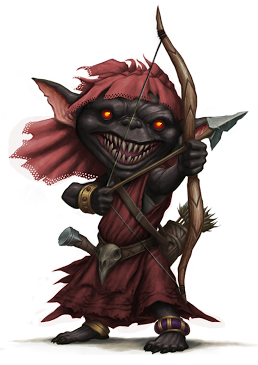
\includegraphics[width=80mm]{./content/img/exme1.png}
\begin{figure}[h]
\end{figure}
\end{center}

\subsection*{Details} 

\noindent

Race: 	Goblin \\
Class: 	Artificer \\
Age: 	8 \\
Status: Active 

\subsubsection{Background}

Exmerah ``Exme" Sliokzog was born on her feet two minutes before her brother, Kolo, in the barren wastelands of ``the North".  Growing up as a Goblin was not easy and the two young siblings spent their days being chased by wild animals, causing mischief, and being enslaved by evil overlords.  

Naturally ingenious from birth, Exme took the opportunity to learn all that she could from her captors, rising quickly up through the ranks until she became a full-time workshop assistant.  During this period Exme made several inexplicable advances in the field of electromagnetism, culminating in the production of Velterra's first electric gun.  

The two goblins were taken out of their death by Lazarus whilst launching an audacious escape attempt from their Northen stronghold.  

\subsubsection{Personality and Traits}

Exme was always the more softly spoken of the twins, usually happy to follow Kolo's lead and revel in their mischief.  Having seen all of their family and friends enslaved at a young age, both Goblins developed a burning passion for emancipation and dreamed of a free world.  Whilst Kolo took the stance that emancipation could only be gained by the sharp edge of a blade and that the only good human was a dead one, Exme always recognised that the races could work together towards the brighter future that they both craved.  

Following her maturity into a goblin woman and the loss of Kolo, Exme became more adult and took up casual smoking, although she still retains a sense of naivety due to her relative lack of world experience.   

Whilst confident in her abilities and place in the world, Exme has been known to act with extreme jealousy in the presence of other woman, especially those with any connection to Myron.  

\subsubsection{Relationships}

Exme's main bond has and always will be to her younger twin brother Kolo.  Prior to his death the two had never spent more than an hour apart and the loss led Exme to re-examine her life and discover who she was when she by herself.  

Myron and Exme have been involved in an on-going `will-they, won't they' relationship which is perhaps best outlined in her self-published novelette ``Love doesn't have a height limit".  

Stanri 

Exme is always keen to talk to other tinkerers and scholars forming quick friendships with the Goblin's mentor Ruh'Breks Sensei, Nanduan robot guy, George Myron and gnome inventor.  

Exme cares deeply about her companions and mourns the loss of each one, keeping memories of their corpses and honouring fallen comrades through the naming of her creations.  

\subsubsection{Exme's Story}

Starting off as a timid young goblin girl, Exme soon began to find her feet and became one of the most fearsome fighters the world had ever seen.  

The death of Kolo struck Exme harder than anything she had experienced.  She had to leave the team for a short while to regather her thoughts, during which time she started the ``Delilah Hardstone Engineering School for Talented Yung Wimun''.  The losses of Kolo and later Delilah left deep scars on Exme's heart and strengthened her resolve to emancipate the people from the oppression of the Church.

Exme played a key role in developing and maintaining the technical capabilities of the group, inventing several pieces of equipment for her teammates, outfitting the airship and working to develop capability with Excallibrum.  

During the gods talk, Exme found out that Kolo's soul was trapped with Kalimar and she became determined to find a way to save Kolo from his eternal torment.  

\begin{DndSidebar}{On the Gender of Animals}
Exme has done a lot of work in the field of antrhopolgoy examining the gender of animal pairs found in the wild.  For example, the observation that dogs are men and cats are women was widely accepted as a universal truth and single-handedly advanced the field of anthropology in Velterra by decades.  
\end{DndSidebar}

\clearpage